% 
% Annual Cognitive Science Conference
% Sample LaTeX Paper -- Proceedings Format
% 

% Original : Ashwin Ram (ashwin@cc.gatech.edu)       04/01/1994
% Modified : Johanna Moore (jmoore@cs.pitt.edu)      03/17/1995
% Modified : David Noelle (noelle@ucsd.edu)          03/15/1996
% Modified : Pat Langley (langley@cs.stanford.edu)   01/26/1997
% Latex2e corrections by Ramin Charles Nakisa        01/28/1997 
% Modified : Tina Eliassi-Rad (eliassi@cs.wisc.edu)  01/31/1998
% Modified : Trisha Yannuzzi (trisha@ircs.upenn.edu) 12/28/1999 (in process)
% Modified : Mary Ellen Foster (M.E.Foster@ed.ac.uk) 12/11/2000
% Modified : Ken Forbus                              01/23/2004
% Modified : Eli M. Silk (esilk@pitt.edu)            05/24/2005
% Modified: Niels Taatgen (taatgen@cmu.edu) 10/24/2006

%% Change ``a4paper'' in the following line to ``letterpaper'' if you are
%% producing a letter-format document.

\documentclass[10pt,letterpaper]{article}

\usepackage{cogsci}
\usepackage{pslatex}
\usepackage{graphicx}
\usepackage{float}
\usepackage{placeins}
\usepackage{amsmath}
\usepackage{apacite}


\title{Referential cues modulate attention and memory \\
during cross-situational word learning}
 
\author{{\large \bf Kyle MacDonald} \\ \texttt{kylem4@stanford.edu} \\ Department of Psychology \\ Stanford University
  \And {\large \bf  Daniel Yurovsky} \\ \texttt{yurovsky@stanford.edu} \\ Department of Psychology \\ Stanford University
  \And {\large \bf Michael C. Frank} \\  \texttt{mcfrank@stanford.edu} \\Department of Psychology \\ Stanford University}


\begin{document}

%% TODO:
% How to talk about exclusionary criteria? 
% How to model the data from experiment 3? -- Can I remove interaction term? 
% How to interpret/frame reliability data?

\maketitle

%%%%%%%% ABSTRACT %%%%%%%

\begin{abstract}
Learning the meanings of words is a complex problem that requires learners to solve many interconnected problems. One of these is the problem of referential uncertainty: within an individual naming context word meaning can be largely unconstrained. Recent empirical and modeling work suggests that this problem can be solved by aggregating word-object co-occurrence statistics across naming contexts. But human learners are constrained by limits on attention and memory, and therefore must store a subset of the information available in each learning moment---how do they select what information to store? We hypothesize that the presence of referential cues like eye gaze guides how learners allocate their attention. In three large-scale experiments with adults, we test how the presence of referential cues affects cross situational word learning. Referential cues shift learners away from multiple hypothesis tracking towards storing only a single hypothesis; without referential cues learners track multiple word-object associations (Experiments 1 and 2). In addition, learners are sensitive to the reliability of referential cues and when they are less reliable, they are less likely to store a strong single hypothesis (Experiment 3).  Together, the data suggest a rational tradeoff: In conditions of greater uncertainty, learners tend to store a broader range of information. 

\textbf{Keywords:} 
statistical learning, word learning, referential cues, resource rationality
\end{abstract}

%%%%%%%% INTRO %%%%%%%

\section{Introduction}

Words are powerful tools that allow speakers to rapidly convey meaning. We focus here on the task of mapping concrete nouns to objects, as opposed to other substantive inferential problems such as word segmentation and generalization. To make such a mapping, learners must solve the core problem of referential uncertainty \cite{quine19600}: that a speaker's utterance could refer to many possible objects in the visual scene, to parts of of those objects, or even to something that is not present. How do learners infer word meanings from data with this kind of uncertainty?

Statistical learning theories offer a solution to this learning problem by aggregating cross-situational statistics across labeling events to identify underlying word meanings. Recent experimental work shows that both adults and young infants can use word-object co-occurrence statistics to learn words from individually ambiguous naming events \cite{smith2008infants, vouloumanos2008fine}. For example, \citeA{smith2008infants} taught 12-month-olds three novel words simply by repeating consistent novel word-object pairings across 10 ambiguous exposure trials. Moreover, recent computational models suggest that cross-situational learning can scale up to learn adult-sized lexicons, even under conditions of considerable referential uncertainty \cite{smith2011cross}.

At the computational level, cross-situational word learning proceeds by the learner taking input from the world in the form of co-occurrences between words and objects, and then performing a statistical computation ovxer that input. But there is still debate about the underlying psychological processes that support cross-situational word learning \cite{smith2014unrealized}. While some theories hold that we accumulate graded, statistical evidence about multiple referents for each word \cite{mcmurray2012word}, others suggest that we track only a single candidate referent \cite{trueswell2013propose}, which is either confirmed or disconfirmed by cross-situational statistics.  

% TODO: fix description of Dan and Mike's model 

Recent experimental and modeling work suggests an integrative explanation: that learners store both a strong single hypothesis and weaker alternative hypotheses, depending on attention and memory demands present during learning \cite{yurovsky2014algorithmic}. When these demands are low, learners represent more alternatives; whereas when demands are high, learners do not store much more than their single candidate hypothesis. This pattern of data was not predicted by an ideal learning model, but a resource-limited version of the model was successful in capturing this tradeoff.

One particularly interesting feature of this approach is that it places single vs. multiple hypothesis tracking on a continuum of learning strategies, along which the learner can then flexibly move depending on the learning context. Put another way, \citeA{yurovsky2014algorithmic}'s data suggest that learners are adaptively changing the strength of word-object representations based on a) the quality of the input and b) their limited cognitive resources. This characterization fits well with recent modeling and experimental work that attempts to offer resource-rational explanations of higher cognition \cite{griffiths2014rational}. For example, \citeA{vul2014} showed that as time-pressure increased in a decision-making task, participants were more likely to show behavior consistent with a less cognitively challenging strategy of matching, rather than with the globally optimal strategy. Are there comparable aspects of the word learning context that might shift learners' allocation of cognitive resources?

Here we consider the hypothesis that referential cues (e.g., eye gaze and pointing) modulate learners' resource allocation by providing evidence about the speaker's intended meaning. Social-pragmatic theories of language learning have emphasized referential cues as critical for early word learning  \cite{bloom2002children, clark2009first}. Experimental work shows that even children as young as 16 months are sophisticated intention-readers, preferring to map novel words to objects that are the target of a speaker's gaze and not their own \cite{baldwin1993infants}. And in naturalistic observations, learners tend to retain labels that are accompanied with clear referential cues that are concurrent with visual access \cite{yu2012embodied}. Together, the evidence suggests that referential cues could help learners by allowing for efficient allocation of limited attention to the relevant statistics in the input.

In the current set of studies, we test the effect of referential cues on the number of representations stored during cross-situational word learning. In Experiment 1, we manipulate the presence of a valid referential cue, a speaker's eye gaze, at different levels of attention and memory demands. At all levels of difficulty, learners tracked a strong single hypothesis, but learners were less likely to track multiple word-object links when referential cues were present. In Experiment 2, we replicate the findings from Experiment 1 with a more ecologically valid stimulus set. In Experiment 3, we show that manipulating the validity of the referential cue increases learners multiple hypothesis tracking. Together, the data suggest that learners adaptively allocate attention and store representations with different levels of fidelity depending on the amount of referential uncertainty present during learning.	

%%%%%%%% EXPT 1: Add social cue, manipulate attention/memory %%%%%%%

\section{Experiment 1}

We set out to test the effects of referential cues on cross-situational learning at different levels of attention and memory demands. Participants saw a series of ambiguous word-learning trials that consisted of a set of novel objects (either 2, 4, 6, or 8) and an image of a schematic, female interlocutor. On each trial they heard a novel word that was either paired with an eye gaze cue or not, and were asked to make guesses about which object went with each word. In subsequent test trials, participants heard the novel word again after different numbers of intervening trials (0, 1, 3, and 7), this time paired with another set of novel objects. One of the objects in the set was either the participant's initial guess (Same trials) or one of the objects that was \emph{not} the initial guess (Switch trials). While both single and multiple referent trackers could succeed on Same trials, only participants who encoded multiple objects during their first encounter could succeed on Switch trials. This provides a direct test of whether learners track multiple alternatives and if these representations are influenced by the presence of referential cues. 

\subsection{Methods}

\subsubsection{Participants}

This experiment was posted to Amazon Mechanical Turk as a set of
Human Intelligence Tasks (HITs) to be completed only by participants with US IP
addresses and an approval rate above 95\%. Each HIT paid 30 cents. Approximately 50-75 HITs were posted for each of the 32 conditions (4 referents X 4 intervals X 2 social conditions) for total of approximately 2200 paid HITs. If a participant completed the experiment more than once, he or she was paid each time but only data from the first HITs completion was included in the final data set. In
addition, data was excluded from the final sample if participants did not give correct answers for familiar trials (5 HITs excluded).

\subsubsection{Stimuli}
Figure 1 shows stimuli used in Experiment 1. These stimuli consisted of black and white pictures of familiar and novel objects drawn from the set of 140 first used in \citeA{kanwisher1997locus}, a schematic drawing of a human interlocutor, and audio recordings of familiar and novel words. 
Familiar words consisted of the labels for the familiar objects as produced by AT\&T Natural VoicesTM (voice: Crystal). Novel words were 1--3 syllable pseudowords obeying the rules of English phonotactics produced using the same speech synthesizer. 
A schematic drawing of a human speaker was chosen for ease of manipulating the direction of eye gaze, the social cue of interest in this study (see Figure 1). 

%%%%%%% FIG 1 Stimuli %%%%%%
\begin{figure} [t!]
\begin{center}
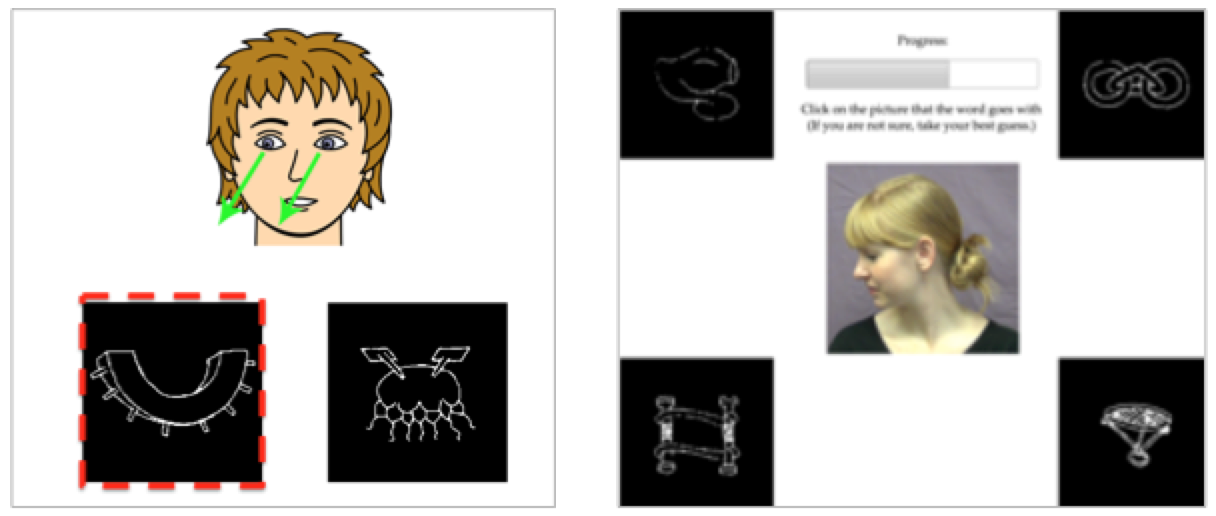
\includegraphics[scale=0.4]{plots_figs/soc-xsit-stimuli.png}
\end{center}
\caption{Experimental stimuli from Experiment 1 (schematic) and Experiment 2 (live action).}
\end{figure}
%%%%%%%%%%%%%%%%%%%%

%%%%%%% Accuracy Plot Expt 1 %%%%%%
\begin{figure*}[t!]
\begin{center}
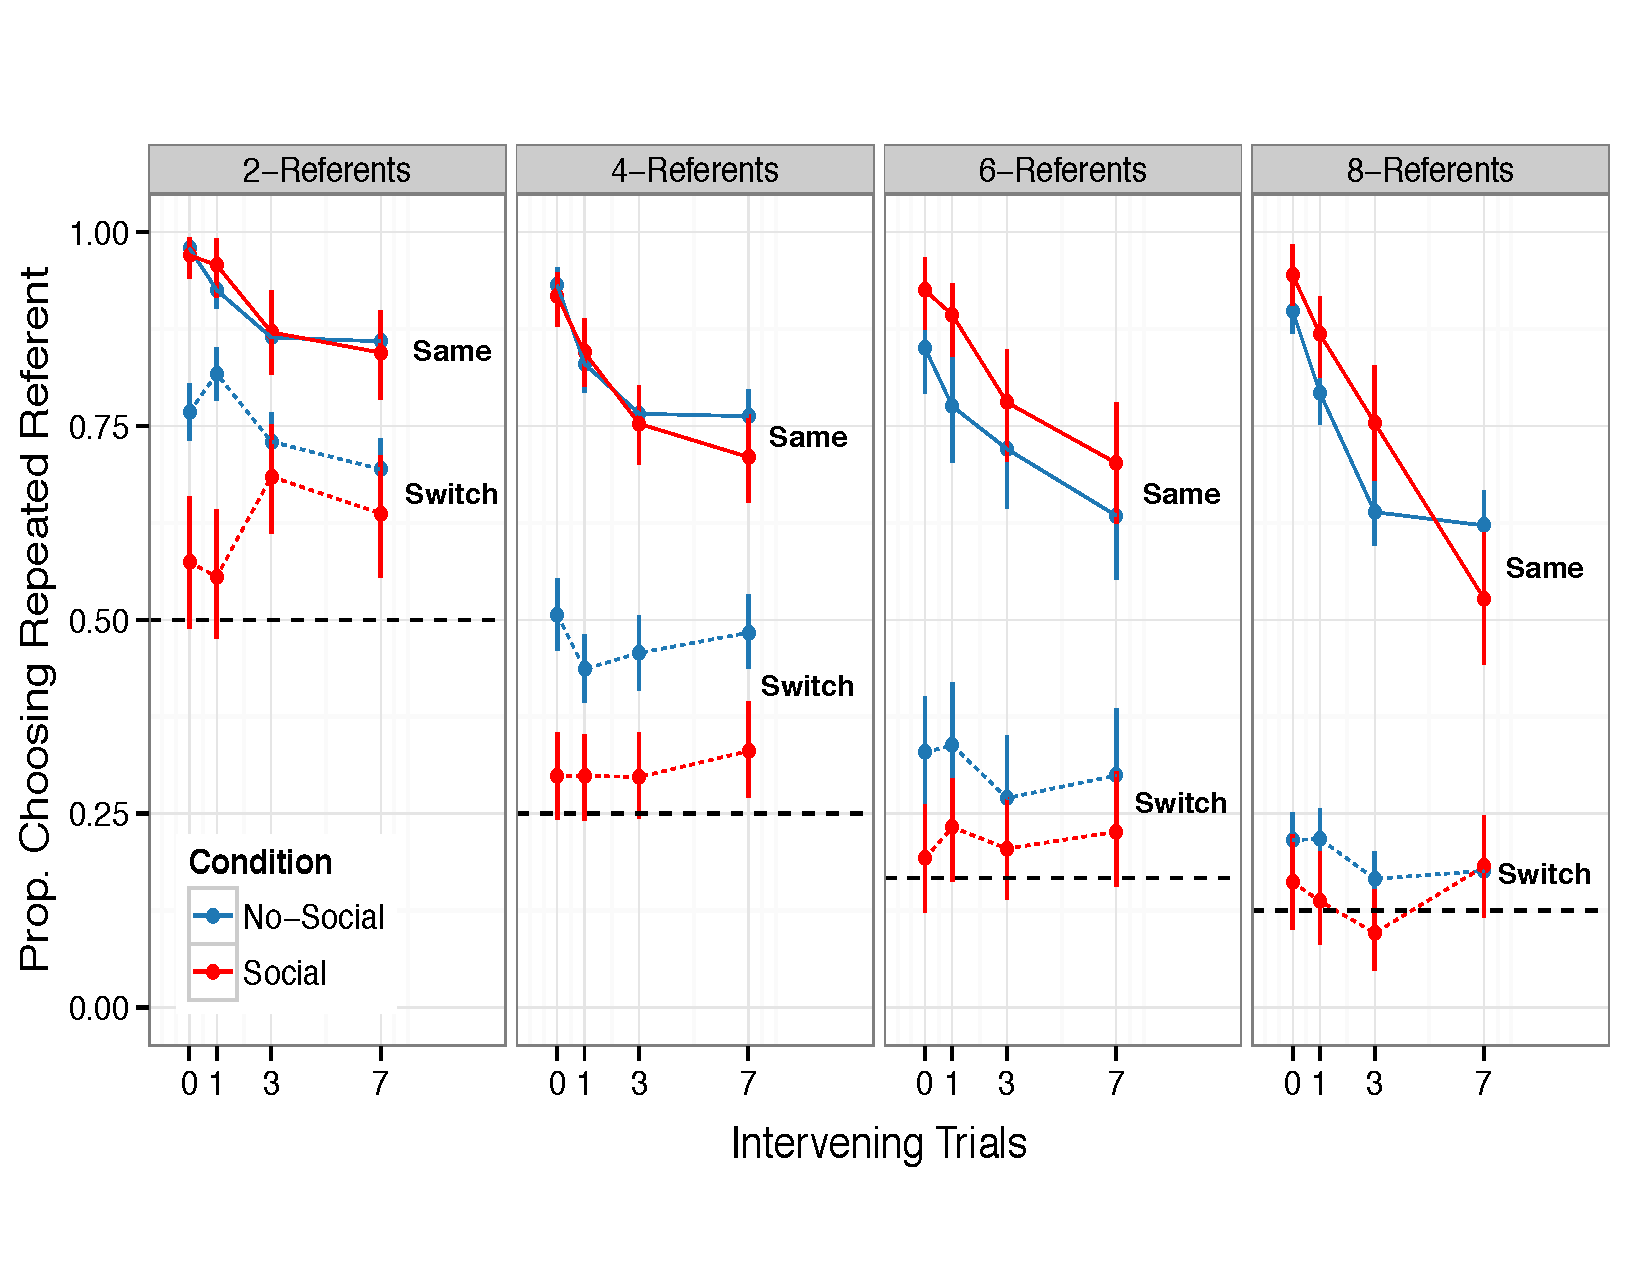
\includegraphics[scale=0.5]{plots_figs/acc-test-expt1}
\end{center}
\caption{Accuracy on test trials in Experiment 1 for both trial types (Same and Switch) and 
experimental conditions (Social and Non-social). Each datapoint represents 
approximately 50-75 participants. Error bars indicate 95\% confidence intervals 
computed by non-parametric bootstrap.}
\end{figure*}
%%%%%%%%%%%%

\subsubsection{Design and Procedure}

Participants were exposed to a series of trials in which they heard a speaker say a novel word, 
saw a set of novel objects, and were asked to guess which object went with the word. 
After a written explanation of the task, participants completed four practice trials that consisted of 
familiar words and objects. These trials also served to screen for participants
who did not have their audio enabled or who were not attending to the task.

After the practice trials, participants were informed that they would now hear
novel words, and see novel objects, and that they should continue selecting the correct
referent for each word. Participants saw either 2, 4, 6, or 8 referents on
the screen and heard eight novel words twice, with either 0, 1, 3, or 7 trials in between exposure and test. Four of the test trials were \textit{Same} trials in which the object that participants selected on the exposure trial appeared again amongst a set of new objects. 
The other four were \textit{Switch} trials in which one of the objects in the set was selected 
randomly from the objects that the participant did not select on the previous exposure trial. 
All other objects were completely novel on each trial. 

Participants were randomly assigned to either the Social or Non-social condition. In the Social condition, eye gaze was directed towards one of the objects on exposure trials; in the Non-social condition, eye gaze was directed straight ahead. On test trials, eye gaze was never informative. To indicate that participants' selections had been registered, a red dashed box appeared around the object they selected for 1 second after their click was received. This box appeared around the selected object whether or not it was the "correct" referent.

\subsection{Results and Discussion}

\subsubsection{Exposure trials}

To ensure that our referential cue manipulation was effective we compared participant's performance on Exposure trials in the Social condition against the distribution expected if participants were selecting randomly (defined by a Binomial distribution with four trials and a probability of success of $\frac{1}{\# Referents}$). In all conditions, participants' responses differed from those expected by chance, exact binomial  $p$(two-tailed) $< .001$, suggesting that eye gaze effectively directed participants' attention to the target referent. 

We also analyzed participants' response times on exposure trials, which were self-paced and thus a proxy for attention allocated to the referents on the screen. We fit a linear mixed effects  model to response times on exposure trials.\footnote{All mixed-effects models were fit using the lme4 package in R. The model was specified as follows: \texttt{RT $\sim$ Condition~$\times$~Log(Interval)~$\times$~Log(Referents) + (Trial Type \textbar~subject)}.} We found a significant main effect of referents ($\beta=  806.88$, $p< .001$) with slower responses as the number of referents increased. We also found a significant 2-way interaction between condition and number of referents ($\beta=  -517.36$, $p< .001$) such that responses were faster in the social condition, especially as the number of referents increased.

%%%%%%%% Exposure Trials Plot Expt 1 %%%%%%
%\begin{figure}[ht]
%\begin{center}
%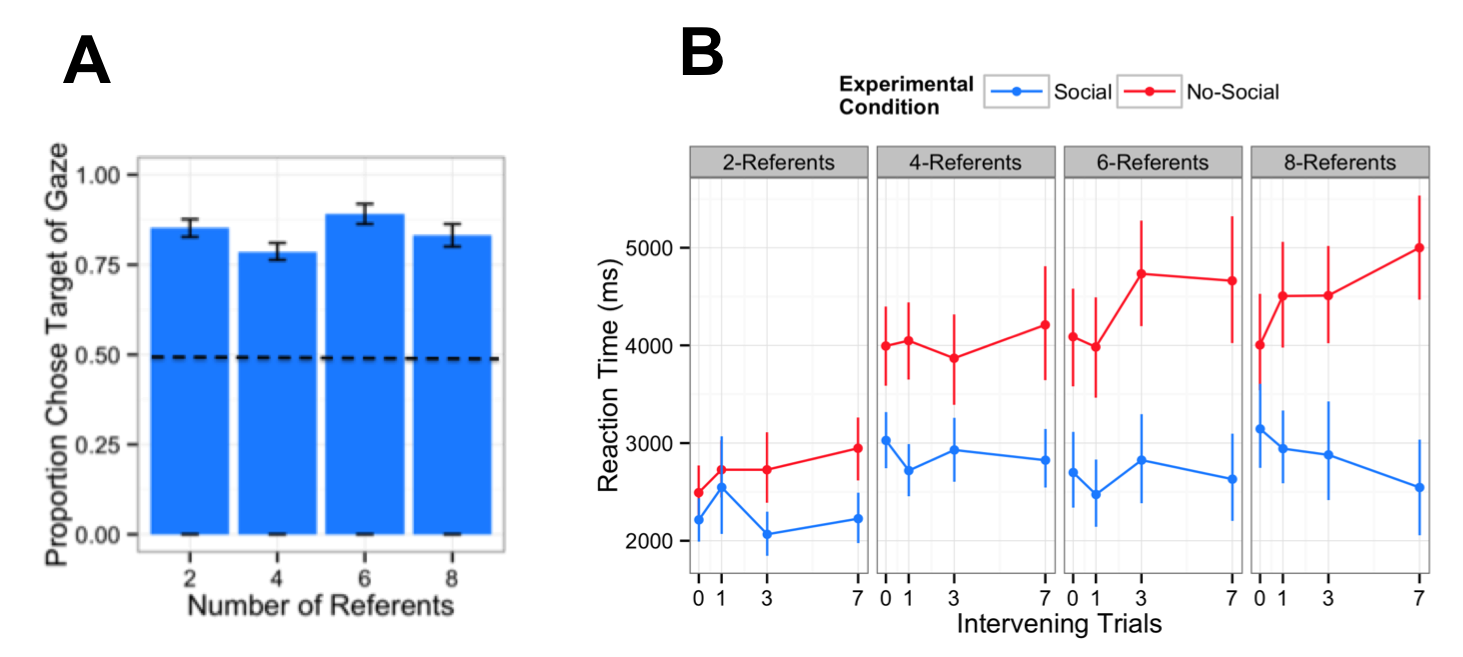
\includegraphics[scale=0.35]{plots_figs/exp_all.png}
%\end{center}
%\caption{Data from exposure trials in Experiment 1. Panel A shows participants' accuracy across the four referent conditions. 
%Participants reliably selected the target of the speaker's eye gaze, suggesting that the social cue was effective. 
%Panel B shows participants' response times on exposure trials. Participants responded faster in the Social condition across all levels of 
%attention and memory demands.}
%\end{figure}
%%%%%%%%%%%%%

\subsubsection{Test trials}

To analyze performance on Test trials, we compared the distribution of correct responses made by each participant to the distribution expected if participants were selecting randomly. Figure 2 shows participants' accuracies in identifying the referent of each word in all conditions for both kinds of trials (Same and Switch) and in each condition (Social and Non-social). We replicate the finding from \citeA{yurovsky2014algorithmic}: at all Referent and Interval levels, both for Same and for Switch trials, participants' responses differed from those expected by chance (smallest $\chi^{2}(4) = 12.07, p < .01$). Thus, learners encoded more than a single hypothesis in ambiguous word learning situations, even under high attentional and memory demands and in the presence of a social cue to reference. 

To quantify the effect of each factor on the likelihood of a correct response, we fit a mixed-effects logistic regression model to the full dataset.\footnote{The model specification was as follows: \texttt{Correct $\sim$ Trial Type~$\times$~Condition~$\times$~Log(Interval)~$\times$~Log(Referents) + (Trial Type \textbar~subject)}.} We found significant main effects of number of referents ($\beta= -0.70$, $p< .001$) and interval ($\beta= -0.60$, $p< .001$), such that as each of these factors increased, accuracy on test trials decreased. We also found significant main effects of trial type ($\beta= -1.56$, $p< .001$) and social condition $\beta= -0.45$, $p< .001$), with worse performance on switch trials and in the social condition. 

Next we examined the interactions between each factor. There were significant two-way interactions between trial type and all three factors: social condition ($\beta= -0.41$, $p< .001$), interval ($\beta= 0.51$, $p< .001$), and number of referents ($\beta=-0.61$, $p< .001$). This analysis shows that a) participants were less accurate on switch trials in the social condition, b) increasing the interval between exposure and test affected same trials more than switch, and c) increasing the number of referents affected switch trials more than same trials. Thus, word learning occurred in all conditions, but switch trials were always more challenging in the social condition.

% latex table generated in R 3.1.2 by xtable 1.7-4 package
% Thu Jan 29 16:10:22 2015
%\begin{table*}[!t]
%\begin{center}
%\caption{Predictor estimates with standard errors and significance information for a logistic mixed-effects model predicting word learning in Experiment 1.} 
%\label{tab:exp1_reg}
%\vskip 0.12in
%\begin{tabular}{lrrrrl}
%\hline
% Predictor & Estimate & Std. Error & $z$ value & $p$ value & stars \\ 
%  \hline
%Intercept & 4.16 & 0.20 & 21.08 & 0.00 & *** \\ 
%  Switch Trial & -1.56 & 0.16 & -9.52 & 0.00 & *** \\ 
%  Social Condition & -0.45 & 0.20 & -2.29 & 0.02 & * \\ 
%  Log(Interval) & -0.60 & 0.08 & -7.73 & 0.00 & *** \\ 
%  Log(Referents) & -0.70 & 0.08 & -8.81 & 0.00 & *** \\ 
%  Switch Trial*Social Condition & -0.41 & 0.09 & -4.40 & 0.00 & *** \\ 
%  Switch Trial*Log(Interval) & 0.51 & 0.04 & 12.31 & 0.00 & *** \\ 
%  Switch Trial*Log(Referent) & -0.61 & 0.06 & -9.92 & 0.00 & *** \\ 
%  Social Condition*Log(Interval) & 0.06 & 0.05 & 1.24 & 0.22 &  \\ 
%  Social Condition*Log(Referent) & 0.14 & 0.07 & 1.84 & 0.07 & . \\ 
%  Log(Interval)*Log(Referent) & 0.01 & 0.03 & 0.17 & 0.87 &  \\ 
%   \hline
%\end{tabular}
%\end{center}
%\end{table*}

Taken together, the response time and accuracy analyses provide support that the presence of a referential cue modulated participants' attention during learning, thus making them less likely to track multiple word-object links. Interestingly, we did not see strong evidence that reduced tracking of alternatives resulted in a boost to participants' performance on same trials. This finding suggests that the limitations on same trials may be different than those regulating the distribution of attention on switch trials, since the presence of a referential cue selectively reduced learners tracking of alternatives but did not lead learners to form a stronger memory of their single candidate hypothesis. 

%%%%%%%% EXPT 2: Improved stimuli %%%%%%%

\section{Experiment 2}

In Experiment 2, we attempt to replicate the findings from Experiment 1 using a more ecologically valid stimuli set. To move closer to a real word learning context, we replaced the schematic stimulus set with a live actress and introduced a within-subjects design where each participant saw both social and non-social learning trials. We additionally selected a subset of conditions, testing only the four-referent display with 0 and 3 intervening trials. Our goals were to replicate the effect of referential cues on learners' multiple hypothesis tracking, and to test whether increasing the ecological validity of the cue would result in a boost to the strength of learners' single candidate hypothesis.  

%%%%%%%% Exposure trials Plot Expt 2 %%%%%%
\begin{figure}[t!]
\begin{center}
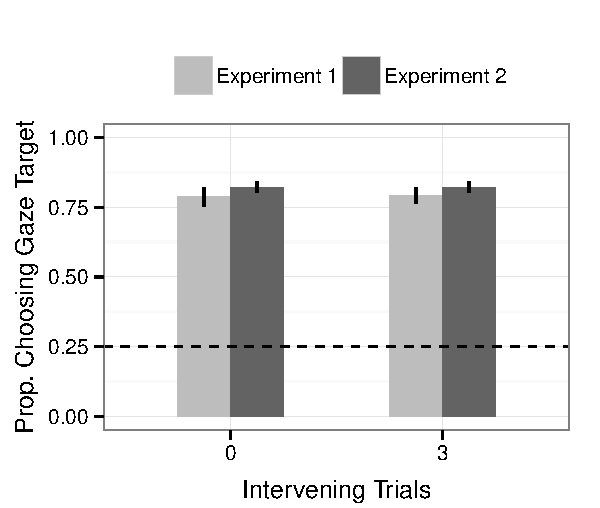
\includegraphics[scale=0.4]{plots_figs/acc-expo-expt1_2}
\end{center}
\caption{Data from exposure trials in Experiments 1 and 2. For comparability with Experiment 2, only data from matching conditions of Experiment 1 are shown. Participants reliably selected the target of the speaker's eye gaze in both experiments, with a small increase in accuracy when the stimulus was a live actress.}
\end{figure}
%%%%%%%%%%%%%

\subsection{Methods}

\subsubsection{Participants}

Participant recruitment, and inclusionary/exclusionary criteria were identical to those of Experiment 1 (excluded 36 HITs). 100 HITs were posted for each condition (1 referent X 2 intervals X 2 social-block conditions) for total of 400 paid HITs.  

\subsubsection{Stimuli}

%%%%%%% Accuracy Plot Expt 2 %%%%%%
\begin{figure}[t!]
\begin{center}
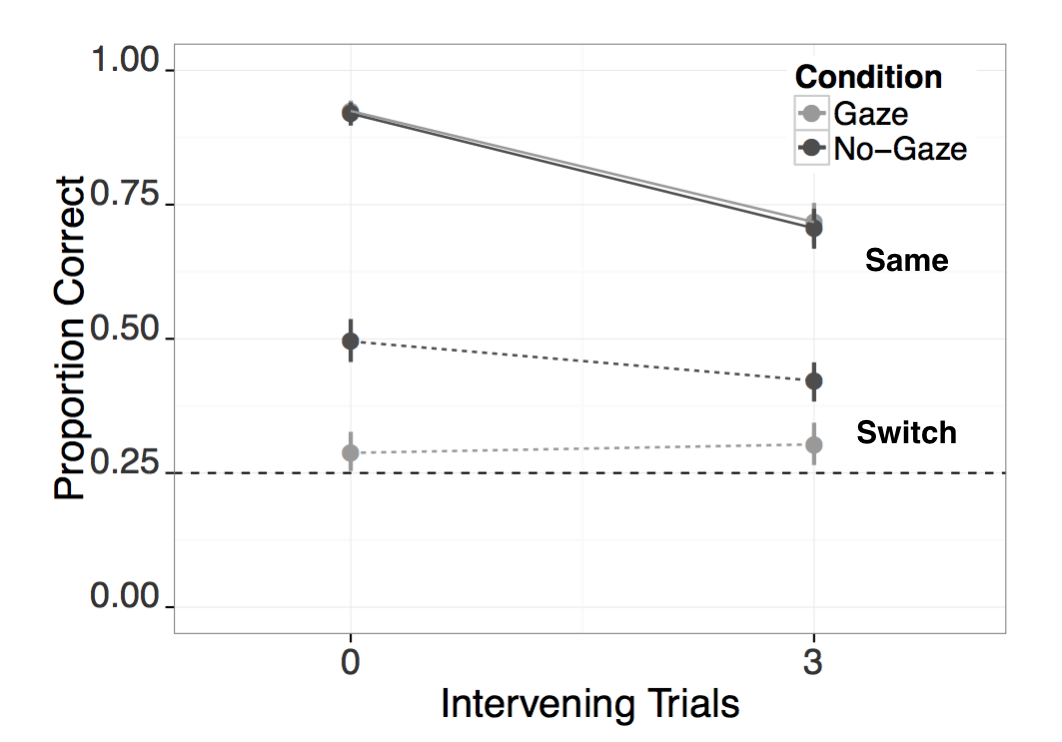
\includegraphics[scale=0.45]{plots_figs/acc-test-expt2}
\end{center}
\caption{Accuracy on test trials in Experiment 2. Each datapoint represents 182 participants. Error bars indicate 95\% confidence intervals computed by non-parametric bootstrap.}
\end{figure}
%%%%%%%%%%%%

Audio and picture stimuli were identical to Experiment 1. The referential cue in the social condition was a film of a live actress (see Figure 1). On each exposure trial, the actress looked out at the participant with a neutral expression, smiled, and then turned to look at one of the four images on the screen. She maintained her gaze for 3 seconds before returning to the center, looking out at the participant. On test trials, she looked straight ahead for the duration of the trial. 

\subsubsection{Design and Procedure}

Procedures were identical to those of Experiment 1. The major design change was a within-subjects manipulation of social cue. That is, participants saw exposure trials with and without eye gaze. The experiment consisted of 2 blocks of 8 trials with 4 same trials and 4 switch trials in each block. Each block contained only social or non-social exposure trials. If the first 8 trials consisted of all social exposure trials, the second 8 trials were all non-social exposure trials. The order of block presentation was counterbalanced across participants. 

\subsection{Results and Discussion}

We followed the same analysis plan as in Experiment 1. First, we analyze performance on exposure trials to ensure that participants were using the referential cue and to test if the cue changed response times. Then we analyze performance on test trials to measure the effect of  the presence of referential cues on the number of word-object links learners stored in memory.

\subsubsection{Exposure trials}

Similar to Experiment 1, participants' responses on exposure trials differed from those expected by chance, exact binomial  $p$(two-tailed) $< .001$, suggesting that eye gaze effective in directing attention to the target referent. Participants in Experiment 2 were slightly more consistent in their use of eye gaze with the live action stimuli in Experiment 2 compared to the schematic stimuli used in Experiment 1 (see Figure 3). We also fit a linear mixed effects  model to response times with the same specification as Experiment 1, finding main effects for social condition ($\beta=  -1112.83$, $p< .001$) and interval ($\beta=  -498.96 $, $p< .001$) with faster responses in the social condition and at the longer interval. The 2-way interaction between social condition and interval was not significant.

%%%%%%%% Exposure trials Plot Expt 2 %%%%%%
%\begin{figure}[h]
%\begin{center}
%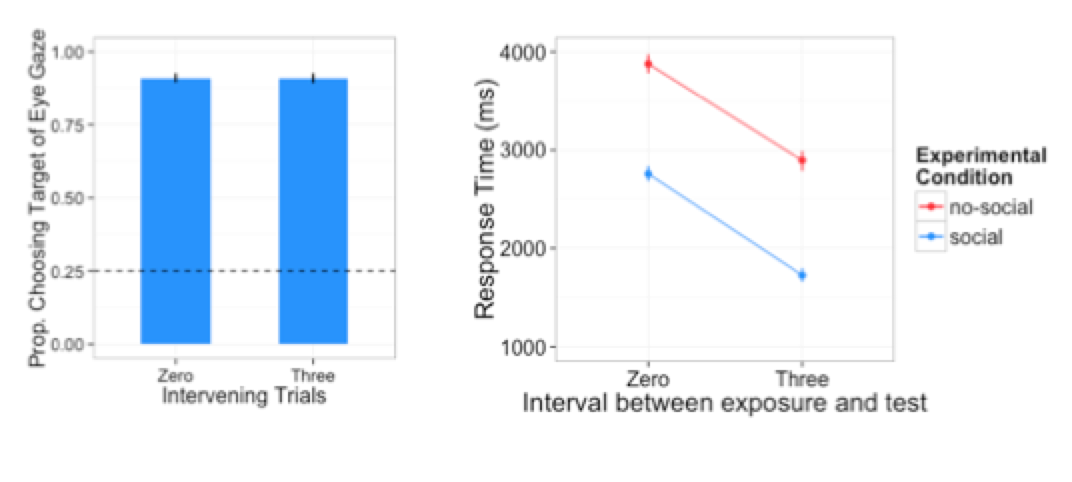
\includegraphics[scale=0.45]{plots_figs/expo_expt2}
%\end{center}
%\caption{Data from exposure trials in Experiment 2. Participants reliably selected the target of the speaker's eye gaze and responded faster in the Social condition.}
%\end{figure}
%%%%%%%%%%%%%

\subsubsection{Test trials}

Figure 4 shows performance on test trials in Experiment 2. We replicate the main finding from Experiment 1: participants in the social condition performed worse on switch trials. We fit a mixed-effects logistic regression model and found significant main effects of interval ($\beta=  -0.55$, $p< .001$) and trial type ($\beta=  -2.63$, $p< .001$). Participants were less accurate as the interval increased and on switch trials. In addition, the model showed significant 2-way interactions between social condition and trial type ($\beta=  -0.959701$, $p< .001$) such that switch trials were more difficult after social exposure trials. Once again, we did not find evidence of a boost to performance on same trials in the social condition. 

Taken together, the data from Experiment 1 and 2 suggest that the presence of a referential cue reliably shifts learners towards single hypothesis tracking strategy. Changing to a live action stimulus set led to slightly higher rates of participants selecting the target of eye gaze on exposure trials, but did not result in a boost to performance on Same trials, providing additional evidence that the fidelity of participants' single hypothesis was unaffected by the presence of a referential cue.

%%%%%%%% EXPT 3: Manipulate reliability of cue %%%%%%%

\section{Experiment 3}

In Experiment 3, our goal was to move beyond manipulating the mere presence of a referential cue to a parametric manipulation of the strength of that cue. To accomplish this, we varied the reliability of eye gaze as a cue to reference. This design was inspired by experimental work showing that children are sensitive to the past reliability of those around them when deciding whom to ask for new information \cite{koenig2004trust}. By parametrically manipulating reliability, we hoped to measure graded changes in learners' single and multiple hypothesis tracking at different points along a continuum of referential uncertainty.

\subsection{Methods}

\subsubsection{Participants}
Participant recruitment, and inclusionary/exclusionary criteria were identical to those of Experiment 1 (excluded XXX HITs). 50 HITs were posted for each reliability level (0\%, 25\%, 50\%, 75\%, and 100\% ) for total of 250 paid HITs.  

\subsubsection{Design and Procedure}

Procedures were identical to those of Experiment 1 and 2. We modified our cross-situational learning paradigm to include a block of 8 familiarization trials, which established the reliability of the referential cue. To establish reliability, we varied the proportion of same/switch trials that occurred during this familiarization block.\footnote{Switch trials provide evidence that eye gaze is not a reliable predictor of the object that will appear at test.} Participants either saw a) 0, 2, 4, 6, or 8 same trials. After the familiarization block, participants completed a block of 8 test trials. Importantly, since we were no longer testing the effect of presence or absence of referential cues, all exposure trials in Experiment 3 included eye gaze, but this cue was more or less reliable depending on the familiarization block.

%%%%%%% Accuracy Plot Expt 3 %%%%%%
\begin{figure}[t!]
\begin{center}
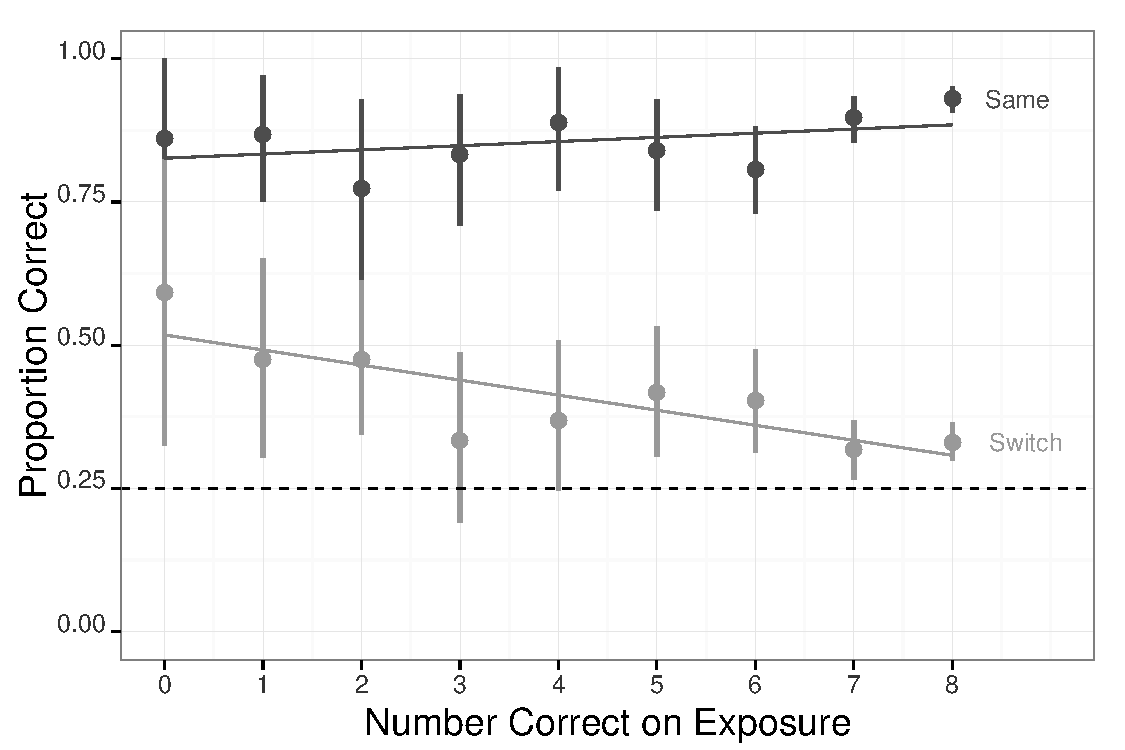
\includegraphics[scale=0.35]{plots_figs/acc-test-expt3}
\end{center}
\caption{Accuracy on test trials in Experiment 3 for both trial types (Same and Switch) at different levels of reliability. Each datapoint represents 
approximately 50 participants. Error bars indicate 95\% confidence intervals 
computed by non-parametric bootstrap.}
\end{figure}
%%%%%%%%%%%%


\subsection{Results and Discussion}

\subsubsection{Exposure trials}
Participants reliably chose the referent that was the target of eye gaze at rates greater than those that would be predicted by chance. When the referential cue was unreliable, in the 0\% reliable condition, participants were less likely to choose the target of gaze, providing evidence of sensitivity to the reliability of the cue. 


%%%%%%%% Acc Exposure Expt 3 %%%%%%
%\begin{figure}[H]
%\begin{center}
%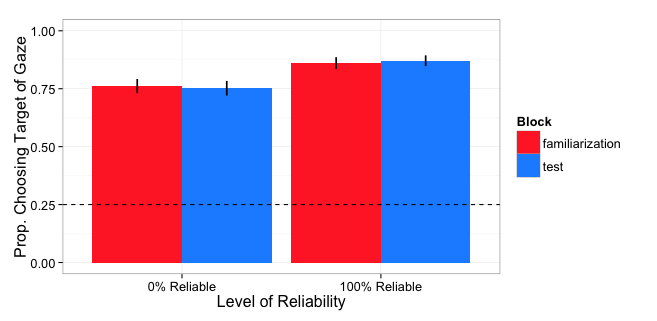
\includegraphics[scale=0.3]{plots_figs/acc-expo-expt3.png}
%\end{center}
%\caption{Accuracy on exposure trials for both familiarization and test blocks in Experiment 3.}
%\end{figure}
%%%%%%%%%%%%%

%%%%%%%% Acc Test Expt 3 %%%%%%
%\begin{figure}[H]
%\begin{center}
%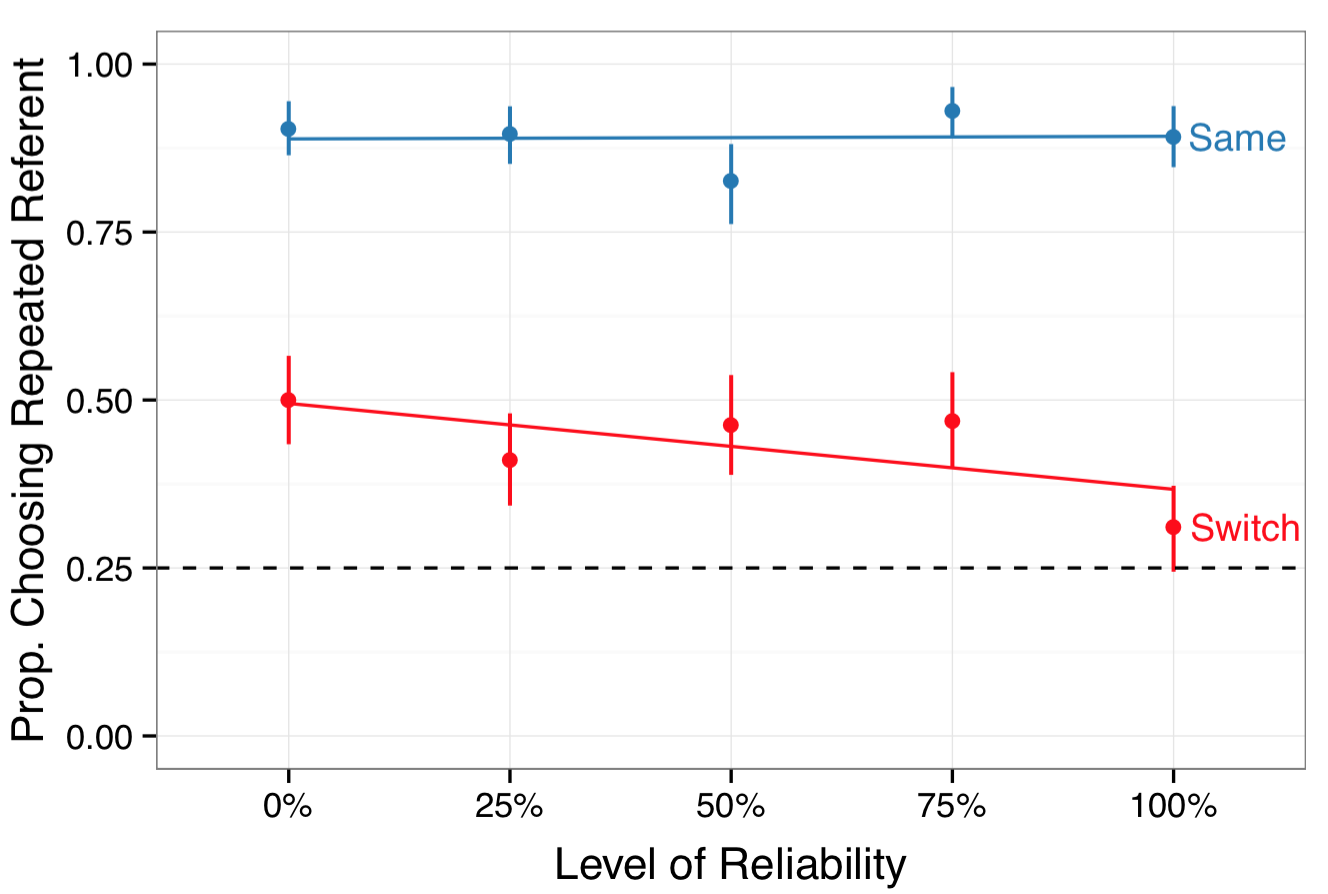
\includegraphics[scale=0.37]{plots_figs/acc-test-expt3.png}
%\end{center}
%\caption{Accuracy on test trials in Experiment 3.}
%\end{figure}
%%%%%%%%%%%%%

\subsubsection{Test trials}
Figure 7 shows participants accuracy on test trials within the test block.  We fit a mixed-effects logistic regression model, which showed significant main effects of Trial Type and Condition.  Participants were less accurate on Switch and in the 0\% Reliable condition. In addition, the model showed a significant two-way interaction between Reliability and Trial Type such that participants performed worse on Same trials in the 0\% Reliable condition. 

\section{General Discussion}

An ideal learner with unlimited attention and memory could track all possible word-object co-occurrences, making cross-situational word learning a simple problem of getting enough data points. But human learners are constrained by limited cognitive resources, making it important to decide which statistics to store from a learning moment. Recent work suggests that learners store a strong candidate hypothesis along with other possible word-object links with varying degrees of fidelity depending on the attention and memory demands present during learning \cite{yurovsky2014algorithmic}. 

In the current line of work, we extend these findings to show that an ecologically valid referential cue to word meaning---the speaker's eye gaze---focuses learners' attention and reduces the attention and memory allocated to other possible word-object links (Experiments 1 and 2). We also parametrically manipulated the reliability of the referential cue, and found that learners showed evidence of multiple hypothesis tracking at all levels of reliability except when the cue was 100\% reliable (Experiment 3). Interestingly, across all three experiments, reduced memory for alternative hypotheses did not result in a boost to performance on same trials. This pattern of data suggests that the presence of a referential cue selectively affected the number of word-object links stored in a given learning moment, but did not strengthen learners' memory for their candidate hypothesis. 

There are several limitations to the current study that are worth noting. First, the social context we used was relatively impoverished. Here we isolated just a single cue to reference, eye gaze, using both a schematic and live action stimulus set. But real-world learning contexts are much more complex, providing learners access to multiple cues to reference such as eye gaze, pointing, and previous discourse. In fact, we did see a more reliable effect of referential cues when we used a live film, which included both eye gaze and head turn as opposed to the static, schematic stimuli. Second, we do not yet know how these results would generalize to young word learners. It is an interesting open question as to how children, who have even more limited cognitive resources, choose to allocate them during learning.

Our results fit well within a resource rational framework \cite{griffiths2014rational}, which attempts to push the rationality of computational-level models down to the psychological process level. In this framework, cognitive systems are thought to be adaptive in that they optimize the use of their limited resources, taking the cost of computation (e.g., opportunity cost of time, metabolic energy, or mental opportunity) into account. In the current work, learners showed evidence of adapting to the level of referential uncertainty in the learning context,  changing how many word-object links they stored in memory.  Thus, understanding how cognitive constraints interact with learners' sensitivity to the sampling process is a promising area for future work.

Word learning proceeds despite the potential for high levels of referential uncertainty and learners' limited cognitive resources. Our work shows how referential cues can influence the allocation of cognitive resources, causing learners to store different numbers of word-object links from a labeling moment. A promising area for future work is to understand how different combinations of input at different levels of referential uncertainty influence individual learning strategies. Overall, these results increase our understanding of how the social-communicative contexts supports language acquisition. 

\section{Acknowledgments}

We are grateful to the members of the Language and Cognition Lab for their feedback on this project. This work was supported by a National Science Foundation Graduate Research Fellowship to KM and an NIH NRSA Postdoctoral Fellowship to DY.


\bibliographystyle{apacite}

\setlength{\bibleftmargin}{.125in}
\setlength{\bibindent}{-\bibleftmargin}

\bibliography{soc-xsit}

\end{document}
